%% -*- mode: LaTeX; TeX-master: "../Summer14.tex" -*-
\section{Combination of upper limits on \mtau LFV branching fractions}
\label{sec:tau:lfv-comb}
\newcommand{\cls}{\ensuremath{\text{CL}_s}\xspace}
\newcommand{\clsb}{\ensuremath{\text{CL}_{s+b}}\xspace}
\newcommand{\clb}{\ensuremath{\text{CL}_b}\xspace}

Combining upper limits is a delicate issue, since there is no standard and
generally agreed procedure. Furthermore, the \mtau LFV searches
published limits are extracted from the data with a variety of
methods, and cannot be directly combined with a uniform procedure. It
is however possible to use a single and effective
upper limits combination procedure for all modes by re-computing the published upper
limits with just one extraction method, using the published
information that documents the upper limit determination:
number of observed candidates, expected background, signal efficiency and
number of analyzed \mtau decays.

We chose to use the \cls method~\cite{Read:2002hq} to re-compute the
\mtau LFV upper limits, since it is well known and widely used (see the
Statistics review of PDG 2013), and since the
limits computed with the \cls method can be combined in a straightforward
way (see below). The \cls method is based on two hypotheses: signal plus background and
background only. We calculate the observed confidence levels for the two
hypotheses:
\begin{align}
&\clsb = P_{s+b}(Q \leq Q_{obs}) = \int_{- \infty}^{Q_{obs}} \frac{dP_{s+b}}{dQ} dQ,
\label{eq:tau:clspdf1} \\
&\clb = P_{b}(Q \leq Q_{obs}) = \int_{- \infty}^{Q_{obs}} \frac{dP_{b}}{dQ} dQ,
\label{eq:tau:clspdf2}
\end{align}
where \clsb is the confidence level observed for the signal plus background
hypothesis, \clb is the confidence level observed for the background only
hypothesis, $\frac{dP_{s+b}}{dQ}$ and $\frac{dP_{b}}{dQ}$ are the probability
distribution functions (PDFs) for the two corresponding hypothesis and
$Q$ is called the test statistics. The \cls value is defined as the ratio
between the confidence level for the signal plus background hypothesis to
the confidence level for the background hypothesis:
\begin{align}
\cls = \dfrac{\clsb}{\clb}.
\end{align}
When multiple results are combined, the PDFs in
Equations~\ref{eq:tau:clspdf1} and \ref{eq:tau:clspdf2} are the
product of the individual PDFs,
\begin{align}
\cls = \dfrac{\prod_{i=1}^{N_{\text{chan}}}\sum_{n=0}^{n_i} \dfrac{e^{-(s_i+b_i)} (s_i+b_i)^{n}}{n!} }{\prod_{i=1}^{n_{\text{chan}}}  \sum_{n=0}^{n_i} \dfrac{e^{-b_i} b_i^{n}}{n!}}    \dfrac{\prod_{j=1}^{n} s_iS_i(x_{ij})+b_iB_i(x_{ij})}{\prod_{j=1}^{n_i}B_i(x_{ij})}~,
\end{align}
where $N_{\text{chan}}$ is the number of results (or channels), and, for each channel $i$,
$n_i$ is the number of observed candidates, $x_{ij}$ are the values of the
discriminating variables (with index $j$), $s_i$ and $b_i$ are the number
of signal and background events and $S_i$, $B_i$ are the probability
distribution functions of the discriminating variables.
The expected signal $s_i$ is related to the \mtau lepton branching
fraction $\BR(\tau \rightarrow f_i)$ into
the searched final state $f_i$ by $s_i = N_i\epsilon_i\BR(\tau \rightarrow
f_i)$, where $N_i$ is the number of produced \mtau leptons and
$\epsilon_i$ is the detection efficiency for observing the decay $\tau\to
f_i$. For $e^+ e^-$ experiments,
$N_i = 2\mathcal{L}_i\sigma_{\tau\tau}$, where $\mathcal{L}_i$ is the
integrated luminosity and $\sigma_{\tau\tau}$ is the
\mtau pair production cross section $\sigma(e^+ e^- \rightarrow \tau^+
\tau^-)$~\cite{Banerjee:2007is}.
In experiments where \mtau leptons are produced in more complex multiple
reactions, the effective $N_i$ is typically estimated with Monte Carlo simulations
calibrated with related data yields.

The extraction of the upper limits is performed using the code provided by
Tom Junk~\cite{junk:2007:cdfnote}. The systematic uncertainties are modeled
in the Monte Carlo toy experiments by convolving the $S_i$ and $B_i$
PDFs with with Gaussian distributions corresponding to the nuisance
parameters. 

Table~\ref{tab:tau:lfv-upper-limits-comb} reports the re-computed limits
for the $B$ factories results as well as the corresponding HFAG
combination. Since there is negligible gain in combining limits of very
different strength, the combinations do not include the CLEO searches and we do not
combine results for modes where the best limit is more than an order of
magnitude better than the other limits.
Figure~\ref{fig:tau:lfv-limits-plot-average} reports the re-computed \mtau
LFV searches upper limits and their combination.

\begin{center}\smaller
\begin{longtable}{lcl@{}rlrrrrrr}
\caption{Combinations of upper limits on lepton flavor violating \mtau decay
  modes. The table includes, for each experimental result, the published information that
  has been used to re-compute the limit with the \cls method, \ie\
  the integrated luminosity, the cross-section for \mtau lepton pairs production,
  the detection efficiency, the number of expected background events and the number
  of observed events. Since the \lhcb collaboration published a limit determined
  with the \cls method, in this case only the published limit is reported.
  The table finally reports the combined limit that is obtained by combining the
  re-computed limits. The modes are grouped according to the particle content of their final
  states. Modes with lepton number violation are labeled with ``(L)'',
  modes with baryon number violation are labeled with ``(BNV)''.
\label{tab:tau:lfv-upper-limits-comb}}%
\\
\toprule
\multicolumn{1}{l}{\bfseries Decay mode} &
\multicolumn{1}{c}{\bfseries Cat.} &
\multicolumn{2}{c}{\bfseries \begin{tabular}{@{}c@{}}90\% CL\\Limit\end{tabular}} &
\multicolumn{1}{c}{\bfseries Exp.} &
\multicolumn{1}{c}{\bfseries \begin{tabular}{@{}c@{}}{\cal L}\\($\text{fb}^{-1}$)\end{tabular}} &
\multicolumn{1}{c}{\bfseries \begin{tabular}{@{}c@{}}$\sigma_{\tau\tau}$\\(nb)\end{tabular}} &
\multicolumn{1}{c}{\bfseries \begin{tabular}{@{}c@{}}efficiency\\(\%)\end{tabular}} &
\multicolumn{1}{c}{\bfseries $N_{\text{bkg}}$} &
\multicolumn{1}{c}{\bfseries $N_{\text{obs}}$} \\
\midrule
\endfirsthead
\multicolumn{5}{c}{{\bfseries \tablename\ \thetable{} -- continued from previous page}} \\
\midrule
\multicolumn{1}{l}{\bfseries Decay mode} &
\multicolumn{1}{c}{\bfseries Cat.} &
\multicolumn{2}{c}{\bfseries \begin{tabular}{@{}c@{}}90\% CL\\Limit\end{tabular}} &
\multicolumn{1}{c}{\bfseries Exp.} &
\multicolumn{1}{c}{\bfseries \begin{tabular}{@{}c@{}}{\cal L}\\($\text{fb}^{-1}$)\end{tabular}} &
\multicolumn{1}{c}{\bfseries \begin{tabular}{@{}c@{}}$\sigma_{\tau\tau}$\\(nb)\end{tabular}} &
\multicolumn{1}{c}{\bfseries \begin{tabular}{@{}c@{}}efficiency\\(\%)\end{tabular}} &
\multicolumn{1}{c}{\bfseries $N_{\text{bkg}}$} &
\multicolumn{1}{c}{\bfseries $N_{\text{obs}}$} \\
\midrule
\endhead
%
%  l\gamma
%  
\begin{ensuredisplaymath}
\Gamma_{156} =  {e^- \gamma} 
\end{ensuredisplaymath}
 &\(\ell\gamma\) & \( <\; \) &  \(5.4 \cdot 10^{-8}\)        & HFAG \\
 &            &&& Belle & \htuse{g156.belle.row} \\
 &            &&& \babar & \htuse{g156.babar.row} \\ 
% \midrule
\begin{ensuredisplaymath}
\Gamma_{157} =  {\mu^- \gamma} 
\end{ensuredisplaymath}
 &            & \( <\; \) &  \(5.0 \cdot 10^{-8}\)        & HFAG \\
 &            &&& Belle & \htuse{g157.belle.row} \\
 &            &&& \babar & \htuse{g157.babar.row} \\ 
\midrule
\begin{ensuredisplaymath}
\Gamma_{160} =  {e^- K^0_S} 
\end{ensuredisplaymath}
 & \(\ell P^0 \)  & \( <\; \) & \(1.4 \cdot 10^{-8}\)         & HFAG  \\
 &            &&& Belle  & \htuse{g160.belle.row} \\
 &            &&& \babar   & \htuse{g160.babar.row} \\ 
%\midrule
\begin{ensuredisplaymath}
\Gamma_{161} =  {\mu^- K^0_S} 
\end{ensuredisplaymath}
 &            & \( <\; \) & \(1.5 \cdot 10^{-8}\)         & HFAG  \\
&            &&& Belle  & \htuse{g161.belle.row} \\
 &            &&& \babar   & \htuse{g161.babar.row} \\ 
\midrule
\begin{ensuredisplaymath}
\Gamma_{164} =  {e^- \rho^0} 
\end{ensuredisplaymath}
 &  \(\ell V^0\) & \( <\; \) & \(1.5 \cdot 10^{-8}\)         & HFAG  \\
 &            &&& Belle& \htuse{g164.belle.row} \\
 &            &&& \babar   & \htuse{g164.babar.row} \\ 
%\midrule
\begin{ensuredisplaymath}
\Gamma_{165} =  {\mu^- \rho^0} 
\end{ensuredisplaymath}
 &            & \( <\; \) & \(1.5 \cdot 10^{-8}\)         & HFAG  \\
 &            &&& Belle& \htuse{g165.belle.row} \\
 &            &&& \babar & \htuse{g165.babar.row} \\ 
%\midrule
\begin{ensuredisplaymath}
\Gamma_{168} =  {e^- K^*(892)^0} 
\end{ensuredisplaymath}
 &            & \( <\; \) & \(2.3 \cdot 10^{-8}\)         & HFAG \\
 &            &&& Belle & \htuse{g168.belle.row} \\
 &            &&& \babar   & \htuse{g168.babar.row} \\ 
%\midrule
\begin{ensuredisplaymath}
\Gamma_{169} =  {\mu^- K^*(892)^0} 
\end{ensuredisplaymath}
 &            & \( <\; \) & \(6.0 \cdot 10^{-8}\)         & HFAG \\
 &            &&& Belle & \htuse{g169.belle.row} \\
 &            &&& \babar   & \htuse{g169.babar.row} \\ 
%\midrule
\begin{ensuredisplaymath}
\Gamma_{170} =  {e^- \bar{K}^*(892)^0} 
\end{ensuredisplaymath}
 &            & \( <\; \) & \(2.2 \cdot 10^{-8}\)         & HFAG \\
 &            &&& Belle & \htuse{g170.belle.row} \\
 &            &&& \babar   & \htuse{g170.babar.row} \\ 
%\midrule
\begin{ensuredisplaymath}
\Gamma_{171} =  {\mu^- \bar{K}^*(892)^0} 
\end{ensuredisplaymath}
 &            & \( <\; \) & \(4.2 \cdot 10^{-8}\)         & HFAG  \\
 &            &&& Belle  & \htuse{g171.belle.row} \\
 &            &&& \babar & \htuse{g171.babar.row} \\ 
%\midrule
\begin{ensuredisplaymath}
\Gamma_{176} =  {e^- \phi} 
\end{ensuredisplaymath}
 &            & \( <\; \) & \(2.0 \cdot 10^{-8}\)         & HFAG \\
 &            &&& Belle & \htuse{g176.belle.row} \\
 &            &&& \babar   & \htuse{g176.babar.row} \\ 
%\midrule
\begin{ensuredisplaymath}
\Gamma_{177} =  {\mu^- \phi} 
\end{ensuredisplaymath}
 &            & \( <\; \) &\(6.8 \cdot 10^{-8}\)          & HFAG \\
 &            &&& Belle  & \htuse{g177.belle.row} \\
 &            &&& \babar   & \htuse{g177.babar.row} \\ 
%\midrule
\begin{ensuredisplaymath}
\Gamma_{166} =  {e^- \omega} 
\end{ensuredisplaymath}
 &            & \( <\; \) & \(3.3 \cdot 10^{-8}\)         & HFAG \\
 &            &&& Belle  & \htuse{g166.belle.row} \\
 &            &&& \babar    & \htuse{g166.babar.row} \\ 
%\midrule
\begin{ensuredisplaymath}
\Gamma_{167} =  {\mu^- \omega} 
\end{ensuredisplaymath}
 &            & \( <\; \) & \(4.0 \cdot 10^{-8}\)         & HFAG \\
 &            &&& Belle  & \htuse{g167.belle.row} \\
 &            &&& \babar   & \htuse{g167.babar.row} \\ 
\midrule
\begin{ensuredisplaymath}
\Gamma_{178} =  {e^- e^+ e^-} 
\end{ensuredisplaymath}
 &  \(\ell\ell\ell\)   & \( <\; \) & \(1.4 \cdot 10^{-8}\)         & HFAG \\
 &            &&& Belle  & \htuse{g178.belle.row} \\
 &            &&& \babar    & \htuse{g178.babar.row} \\ 
%\midrule
\begin{ensuredisplaymath}
\Gamma_{181} =  {\mu^- e^+ e^-} 
\end{ensuredisplaymath}
 &            & \( <\; \) & \(1.1 \cdot 10^{-8}\)         & HFAG \\
 &            &&& Belle & \htuse{g181.belle.row} \\
 &            &&& \babar    & \htuse{g181.babar.row} \\ 
%\midrule
\begin{ensuredisplaymath}
\Gamma_{179} =  {e^- \mu^+ \mu^-} 
\end{ensuredisplaymath}
 &            & \( <\; \) & \(1.6 \cdot 10^{-8}\)         & HFAG \\
 &            &&& Belle  & \htuse{g179.belle.row} \\
 &            &&& \babar     & \htuse{g179.babar.row} \\ 
%\midrule
\begin{ensuredisplaymath}
\Gamma_{183} =  {\mu^- \mu^+ \mu^-} 
\end{ensuredisplaymath}
 &            & \( <\; \) & \(1.2 \cdot 10^{-8}\)         & HFAG \\
 &            &&& Belle& \htuse{g183.belle.row} \\
 &            &&& \babar  & \htuse{g183.babar.row} \\ 
 &            & \( <\; \) & \(4.6 \cdot 10^{-8}\)         & \lhcb   \\ 
%\midrule
\begin{ensuredisplaymath}
\Gamma_{182} =  {e^- \mu^+ e^-} 
\end{ensuredisplaymath}
 &            & \( <\; \) & \(8.4 \cdot 10^{-9}\)         & HFAG \\
 &            &&& Belle  & \htuse{g182.belle.row} \\
 &            &&& \babar    & \htuse{g182.babar.row} \\ 
%\midrule
\begin{ensuredisplaymath}
\Gamma_{180} =  {\mu^- e^+ \mu^-} 
\end{ensuredisplaymath}
 &            & \( <\; \) & \(9.8 \cdot 10^{-9}\)         & HFAG \\
 &            &&& Belle & \htuse{g180.belle.row} \\
 &            &&& \babar     & \htuse{g180.babar.row} \\ 
\midrule
\begin{ensuredisplaymath}
\Gamma_{211} =  { \pi^- \Lambda } 
\end{ensuredisplaymath}
 & BNV & \( <\; \) & \(1.9 \cdot 10^{-8}\)                 & HFAG  \\
 &                &&& Belle  & \htuse{g211.belle.row} \\
 &               &&& \babar     & \htuse{g211.babar.row} \\  
%\midrule
\begin{ensuredisplaymath}
\Gamma_{212} =  { \pi^- \bar{\Lambda}} 
\end{ensuredisplaymath}
 &            & \( <\; \) & \(1.8 \cdot 10^{-9}\)         & HFAG \\
 &            &&& Belle  & \htuse{g212.belle.row} \\
 &            &&& \babar     & \htuse{g212.babar.row} \\  
%\midrule
\begin{ensuredisplaymath}
\Gamma_{213} =  { K^- \Lambda } 
\end{ensuredisplaymath}
 &            & \( <\; \) & \(3.7 \cdot 10^{-9}\)         & HFAG \\
 &            &&& Belle  & \htuse{g213.belle.row} \\
 &            &&& \babar     & \htuse{g213.babar.row} \\  
%\midrule
\begin{ensuredisplaymath}
\Gamma_{214} =  { K^- \bar{\Lambda}} 
\end{ensuredisplaymath}
 &            & \( <\; \) & \(2.0 \cdot 10^{-9}\)         & HFAG \\
 &            &&& Belle & \htuse{g214.belle.row} \\
 &            &&& \babar     & \htuse{g214.babar.row} \\  
\bottomrule
\end{longtable}
\end{center}

\begin{figure}[tb]
  \begin{center}
    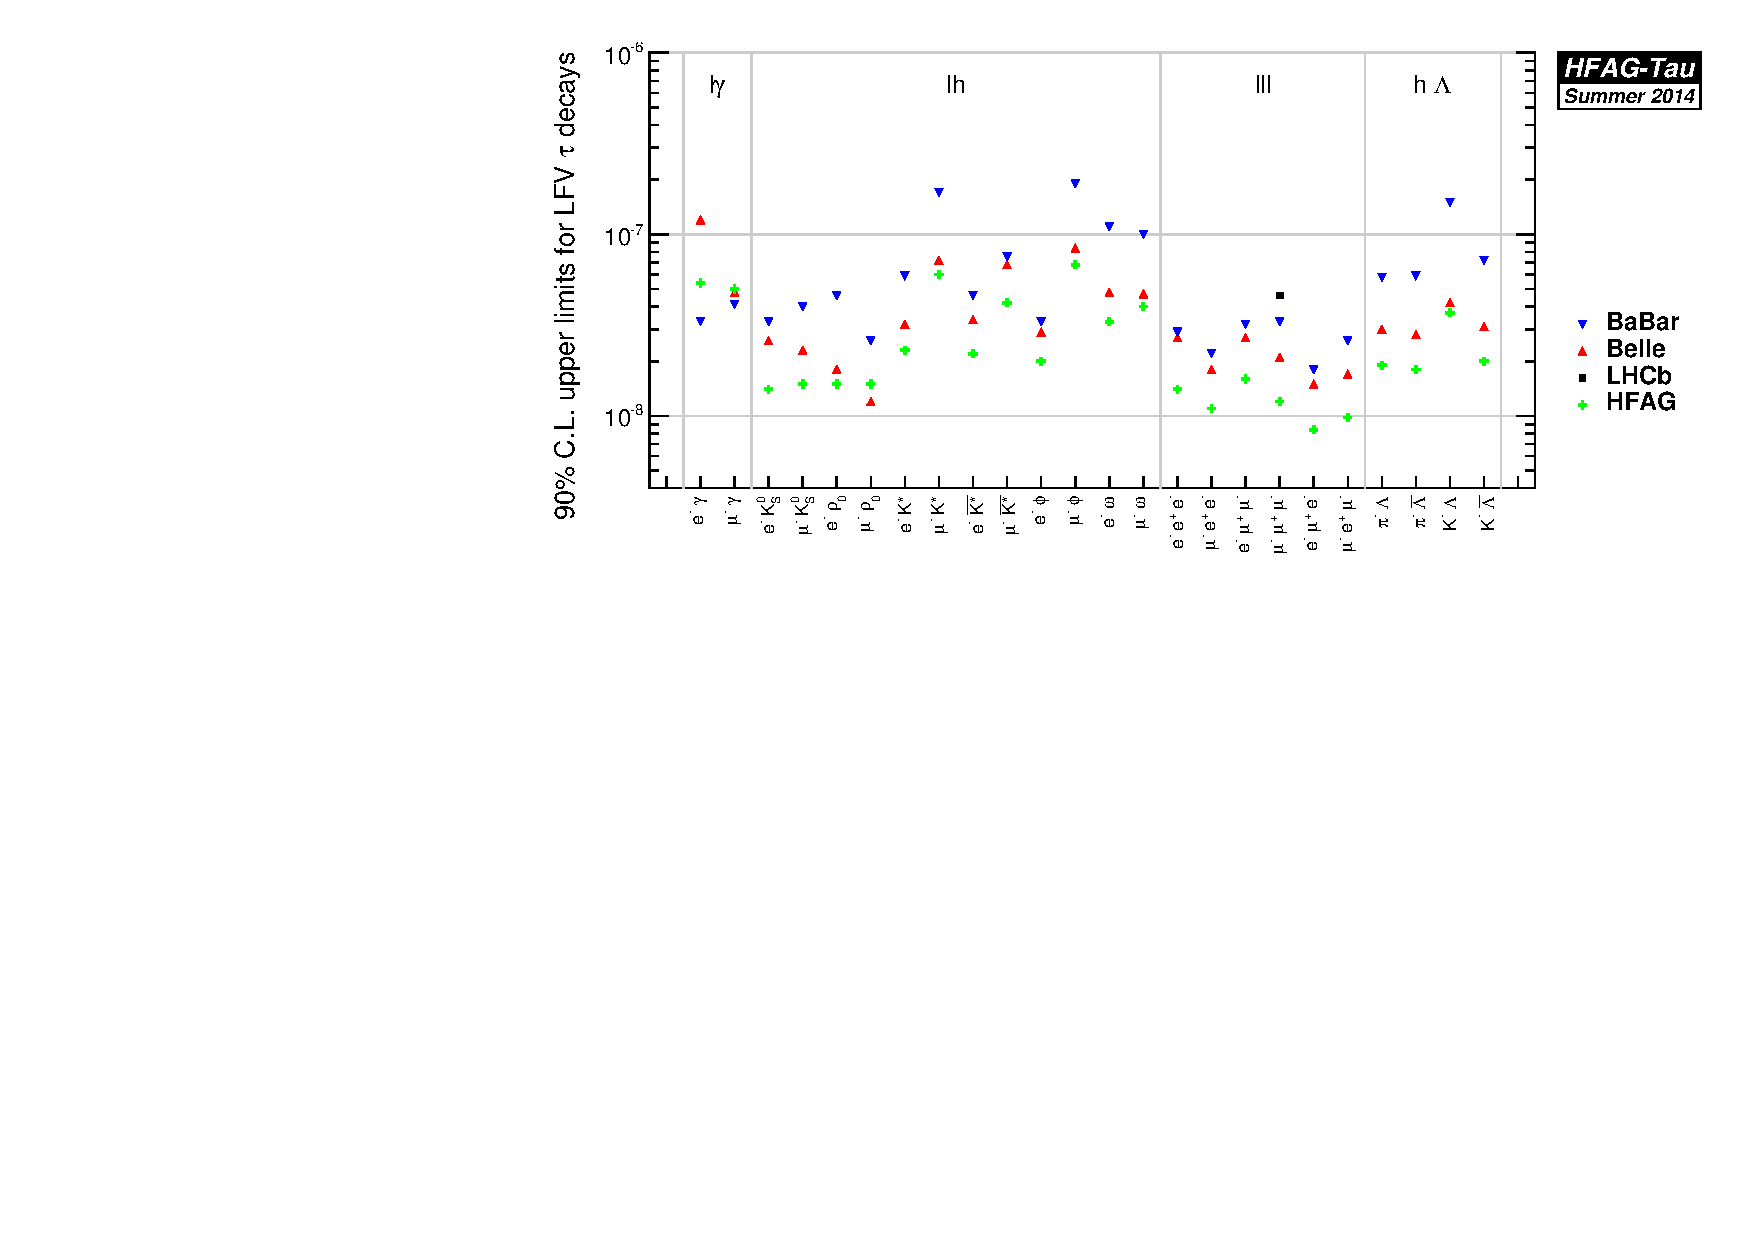
\includegraphics[angle=270,totalheight=0.86\textheight,clip]{TauLFV_combs.pdf}
    \caption{Tau lepton-flavour-violating branching fraction upper limits
      combinations summary plot. For each channel we report the HFAG
      combined limit, and the experimental published limits. In some cases,
      the combined limit is weaker than the limit published by a single
      experiment. This arises since the \cls method used in the
      combination can be more conservative compared to other legitimate
      methods, especially when the number of observed events fluctuates below the
      expected background. 
      \label{fig:tau:lfv-limits-plot-average}
    }
  \end{center}
\end{figure}

%% -*- mode: LaTeX; TeX-master: "../Summer14.tex" -*-
%% ///////////////////////////////////////////////////////////////////////////
